\documentclass[border=10pt]{standalone}
\usepackage{tikz}

\begin{document}

% x-y-z (extrinsic rotations)


% extrinsic rotation

% x phi
\begin{tikzpicture}
    \coordinate (o) at (0,0);
    
    \coordinate (x) at (-2,0);
    \coordinate (y) at (1.4,-1.4);
    \coordinate (z) at (0,2);

    % \draw [->] (o) -- (x) node[left] {$x$};
    \draw [->] (o) -- (y) node[right] {$y$};
    \draw [->] (o) -- (z) node[above] {$z$};
    
    \coordinate (x') at (-2,0);
    \coordinate (y') at (1.5,-.7);
    \coordinate (z') at (-.5,1.8);

    \draw [blue,->] (o) -- (x') node[left] {$x'(x)$};
    \draw [blue,->] (o) -- (y') node[right] {$y'$};
    \draw [blue,->] (o) -- (z') node[above] {$z'$};
    
    
    \coordinate (phiys) at (0.35,-0.35);
    \coordinate (phizs) at (0,0.5);
    \coordinate (phiyl) at (0.32,-0.37);
    \coordinate (phizl) at (-.08,0.47);
    
    \draw (phiys) arc [x radius=.5, y radius=.5, start angle=-45, end angle=-25];
    \draw (phizs) arc [x radius=.5, y radius=.5, start angle=90, end angle=105];
    \node [right,font=\fontsize{5}{5}] at (phiyl) {$\phi$};
    \node [above,font=\fontsize{5}{5}] at (phizl) {$\phi$};
 
\end{tikzpicture}

% y theta
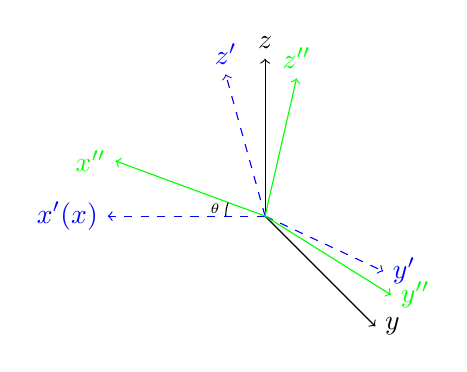
\begin{tikzpicture}
    \coordinate (o) at (0,0);
    
    \coordinate (x) at (-2,0);
    \coordinate (y) at (1.4,-1.4);
    \coordinate (z) at (0,2);

    % \draw [->] (o) -- (x) node[left] {$x$};
    \draw [->] (o) -- (y) node[right] {$y$};
    \draw [->] (o) -- (z) node[above] {$z$};
    
    \coordinate (x') at (-2,0);
    \coordinate (y') at (1.5,-.7);
    \coordinate (z') at (-.5,1.8);

    \draw [dashed,blue,->] (o) -- (x') node[left] {$x'(x)$};
    \draw [dashed,blue,->] (o) -- (y') node[right] {$y'$};
    \draw [dashed,blue,->] (o) -- (z') node[above] {$z'$};
 
    
    \coordinate (x'') at (-1.9,0.7);
    \coordinate (y'') at (1.6,-1.0);
    \coordinate (z'') at (.4,1.75);

    \draw [green,->] (o) -- (x'') node[left] {$x''$};
    \draw [green,->] (o) -- (y'') node[right] {$y''$};
    \draw [green,->] (o) -- (z'') node[above] {$z''$};
    
    \coordinate (thetaxs) at (-0.5,0);
    \coordinate (thetaxl) at (-0.45,.1);
    
    \draw (thetaxs) arc [x radius=.5, y radius=.5, start angle=180, end angle=160];
    \node [left,font=\fontsize{5}{5}] at (thetaxl) {$\theta$};
 
\end{tikzpicture}

% z psi
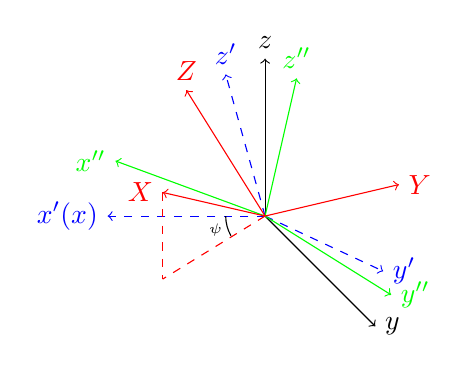
\begin{tikzpicture}
    \coordinate (o) at (0,0);
    
    \coordinate (x) at (-2,0);
    \coordinate (y) at (1.4,-1.4);
    \coordinate (z) at (0,2);

    % \draw [->] (o) -- (x) node[left] {$x$};
    \draw [->] (o) -- (y) node[right] {$y$};
    \draw [->] (o) -- (z) node[above] {$z$};
    
    \coordinate (x') at (-2,0);
    \coordinate (y') at (1.5,-.7);
    \coordinate (z') at (-.5,1.8);

    \draw [dashed,blue,->] (o) -- (x') node[left] {$x'(x)$};
    \draw [dashed,blue,->] (o) -- (y') node[right] {$y'$};
    \draw [dashed,blue,->] (o) -- (z') node[above] {$z'$};
 
    
    \coordinate (x'') at (-1.9,0.7);
    \coordinate (y'') at (1.6,-1.0);
    \coordinate (z'') at (.4,1.75);

    \draw [green,->] (o) -- (x'') node[left] {$x''$};
    \draw [green,->] (o) -- (y'') node[right] {$y''$};
    \draw [green,->] (o) -- (z'') node[above] {$z''$};
    
    
    \coordinate (X) at (-1.3,0.3);
    \coordinate (Xxy) at (-1.3,-0.8);
    \coordinate (Y) at (1.7,.4);
    \coordinate (Z) at (-1,1.6);

    \draw [red,->] (o) -- (X) node[left] {$X$};
    \draw [red,->] (o) -- (Y) node[right] {$Y$};
    \draw [red,->] (o) -- (Z) node[above] {$Z$};
    \draw [red,dashed] (o) -- (Xxy);
    \draw [red,dashed] (X) -- (Xxy);
    
    
    \coordinate (psixs) at (-0.5,0);
    \coordinate (psixl) at (-0.42,-.18);
    
    \draw (psixs) arc [x radius=.5, y radius=.5, start angle=180, end angle=210];
    \node [left,font=\fontsize{5}{5}] at (psixl) {$\psi$};
 
\end{tikzpicture}

\end{document}
